\section{Estimation of the Entanglement Coefficient $\hat\kappa$}
\label{app:kappa_estimation}

% The entanglement coefficient $\kappa(c_u, \rho)$ defined in~\cref{def:overlap} involves the volume of high-dimensional activation regions, which is intractable to compute directly. We instead estimate $\kappa$ using a sample-based procedure to measure the overlap over a neighborhood, which provides us with an estimate lower-bound for the overlap with remaining concepts. Our practical observations indicate that this lower-bound is not lose because the overlap with remaining concepts is mostly dominated by a few concepts. 
The entanglement coefficient $\kappa(c_u, \rho)$ defined in~\cref{def:overlap} involves the volume of high-dimensional activation regions, which is intractable to compute directly. We therefore estimate $\kappa$ via a sample-based procedure that restricts the overlap measurement to a discovered \emph{semantic neighborhood} $\mathcal{N}(c_u) \subseteq \mathcal{C} \setminus \{c_u\}$ rather than the full union over remaining concepts. Because $\mathcal{N}(c_u)$ is a subset of the union appearing in~\cref{def:overlap}, this neighborhood-restricted estimate is a \emph{lower bound} on $\kappa(c_u, \rho)$. 
We argue, and verify in~\cref{app:kappa_per_target}, that this lower bound is tight in practice: across the five targets, the activation overlap with non-neighbors is negligible, so the union over $\mathcal{C} \setminus \{c_u\}$ is dominated by the union over $\mathcal{N}(c_u)$. 
Throughout this section we work with cosine distance $d_{\cos}(\mathbf{a}, \mathbf{b}) = 1 - \langle \mathbf{a}, \mathbf{b} \rangle / (\|\mathbf{a}\|\|\mathbf{b}\|)$, which is the standard choice in representation analysis: it is invariant to activation magnitude (which is dominated by token-position effects under mean-pooling) and captures directional similarity, the property most closely tied to concept identity. 
The centroid-distance matrix used to motivate neighborhood structure in~\cref{sec:tradeoff} (\cref{fig:distance_matrix}) uses the same metric, ensuring internal consistency between our motivation and our formalization.


\paragraph{On the relationship between cosine and $\ell_2$ metrics.}
\Cref{thm:tradeoff} bounds the $\ell_2$ displacement $\|\boldsymbol{\Phi}_{\hat\theta}(p) - \boldsymbol{\Phi}_{\theta}(p)\|_2$, since this quantity measures a physical perturbation to the activation vector. Our $\kappa$ estimator, in contrast, uses cosine distance to characterize region membership. These two choices are compatible: for activations normalized to the unit sphere, $\|\mathbf{a} - \mathbf{b}\|_2^2 = 2 \cdot d_{\cos}(\mathbf{a}, \mathbf{b})$, so an $L$-Lipschitz function under the $\ell_2$ metric is $(L\sqrt{2})$-Lipschitz under cosine distance, and~\cref{asm:lip} transfers directly (with a constant factor absorbed into $L$). 

\paragraph{Activation extraction.}
For each concept $c$, we generate images from 50 shared prompt templates (differing only in the concept word) using the base model (Stable Diffusion v1.4) with DDIM sampling (50 steps, guidance scale 7.5). At step $t^*{=}25$, we extract the cross-attention output at \texttt{mid\_block.attentions.0}, take the text-conditioned component, and mean-pool over spatial dimensions to obtain a single activation vector $\boldsymbol{\Phi}_\theta(p) \in \mathbb{R}^d$ per prompt. 


\paragraph{Neighborhood discovery.}
We restrict the overlap measurement in~\cref{def:overlap} to a finite set of candidate concepts that are close to $c_u$ in activation space. We formalize this set as follows.

\begin{definition}[Semantic neighborhood]
\label{def:semantic_neighborhood}
Let $\mathcal{C}_{\mathrm{pool}} \subset \mathcal{C}$ be a fixed candidate pool shared across targets. For each $c \in \mathcal{C}_{\mathrm{pool}}$, let $\bar{\mathbf{a}}_c = \tfrac{1}{|\mathcal{S}_c|}\sum_{\mathbf{a}\in\mathcal{S}_c}\mathbf{a}$ denote the centroid of its activation samples. Let $\delta > 0$ be a centroid-distance threshold, set in our experiments to the $25$th percentile of the empirical distribution of all pairwise centroid cosine distances $\{d_{\cos}(\bar{\mathbf{a}}_{c_i}, \bar{\mathbf{a}}_{c_j})\}_{c_i \neq c_j \in \mathcal{C}_{\mathrm{pool}}}$, computed once over the full pool and applied uniformly across targets. The \emph{semantic neighborhood} of a target $c_u \in \mathcal{C}_{\mathrm{pool}}$ is
\begin{equation}
    \mathcal{N}(c_u) \;=\; \bigl\{\, c \in \mathcal{C}_{\mathrm{pool}} \setminus \{c_u\} \;:\; d_{\cos}(\bar{\mathbf{a}}_{c_u},\,\bar{\mathbf{a}}_c) \,<\, \delta \,\bigr\}.
\end{equation}
\end{definition}
We emphasize that $\delta$ and $\mathcal{N}(c_u)$ are \emph{estimation-side} constructs: they appear only in the empirical estimator $\hat\kappa$ below and play no role in the theoretical bound of~\cref{thm:tradeoff}, which is stated entirely in terms of $\kappa(c_u, \rho)$. Because $\mathcal{N}(c_u) \subseteq \mathcal{C} \setminus \{c_u\}$, restricting the overlap computation to $\mathcal{N}(c_u)$ yields a lower bound on the true $\kappa$. The discovered neighborhoods are reported in~\cref{tab:kappa_per_target}.


% We define the semantic neighborhood $\mathcal{N}(c)$ using centroid cosine distance. For each pair of concepts $(c_i, c_j)$, we compute the cosine distance between their mean activation vectors $\bar{\mathbf{a}}_{c_i}, \bar{\mathbf{a}}_{c_j}$. We set the neighborhood threshold $\delta$ to the 25th percentile of all pairwise centroid distances: concepts with centroid distance below $\delta$ are considered neighbors. The discovered neighborhoods are reported in~\cref{tab:kappa}.

\paragraph{Overlap estimation.}
For a target concept $c_u$ with discovered neighbors $\mathcal{N}(c_u)$, we estimate $\hat\kappa$ as the fraction of $c_u$'s activation samples that fall within radius $\rho$ of any neighbor's activation samples:
\begin{equation}
    \hat\kappa(c_u) \;=\; \frac{1}{|\mathcal{S}_{c_u}|} \sum_{\mathbf{a} \in \mathcal{S}_{c_u}} \mathbf{1}\!\left[\min_{c' \in \mathcal{N}(c_u)} \min_{\mathbf{b} \in \mathcal{S}_{c'}} d_{\cos}(\mathbf{a}, \mathbf{b}) \leq \rho\right],
\end{equation}
where $\mathcal{S}_c = \{\boldsymbol{\Phi}_\theta(p_i)\}_{i=1}^{50}$ denotes the set of activation samples for concept $c$, and $d_{\cos}$ is the cosine distance. 
The fattening radius $\rho_{c_u}$ is set to the median intra-concept pairwise cosine distance within $c_u$:
\begin{equation}
    \rho_{c_u} \;=\; \mathrm{median}\!\left\{d_{\cos}(\mathbf{a}, \mathbf{a}') \;\middle|\; \mathbf{a}, \mathbf{a}' \in \mathcal{S}_{c_u},\; \mathbf{a} \neq \mathbf{a}'\right\}.
\end{equation}
This choice calibrates the overlap radius to the natural spread of the target concept's activation region: a neighbor activation qualifies as overlapping only if it is as close to some target activation as typical target activations are to each other.

\paragraph{Validation via centroid distance.}
To independently verify that the neighborhoods discovered in the previous step reflect genuine semantic structure rather than noise, we visualize the pairwise centroid cosine distances between all ten concept activation regions. \Cref{fig:distance_matrix} shows the resulting distance matrix, reordered by hierarchical clustering on the centroid distances themselves. Two block structures are immediately visible. The equine cluster (\texttt{horse}$\leftrightarrow$\texttt{pony}: $0.158$; \texttt{horse}$\leftrightarrow$\texttt{donkey}: $0.329$; \texttt{pony}$\leftrightarrow$\texttt{donkey}: $0.271$) 
exhibit small inter-concept distances, 
consistent with the high $\hat\kappa$ values reported in~\cref{tab:kappa}. 
And semantically isolated concepts such as \texttt{castle} have centroid distances exceeding $0.65$ to all animal concepts, consistent with $\hat\kappa \approx 0$.

\begin{figure}[htbp]
\centering
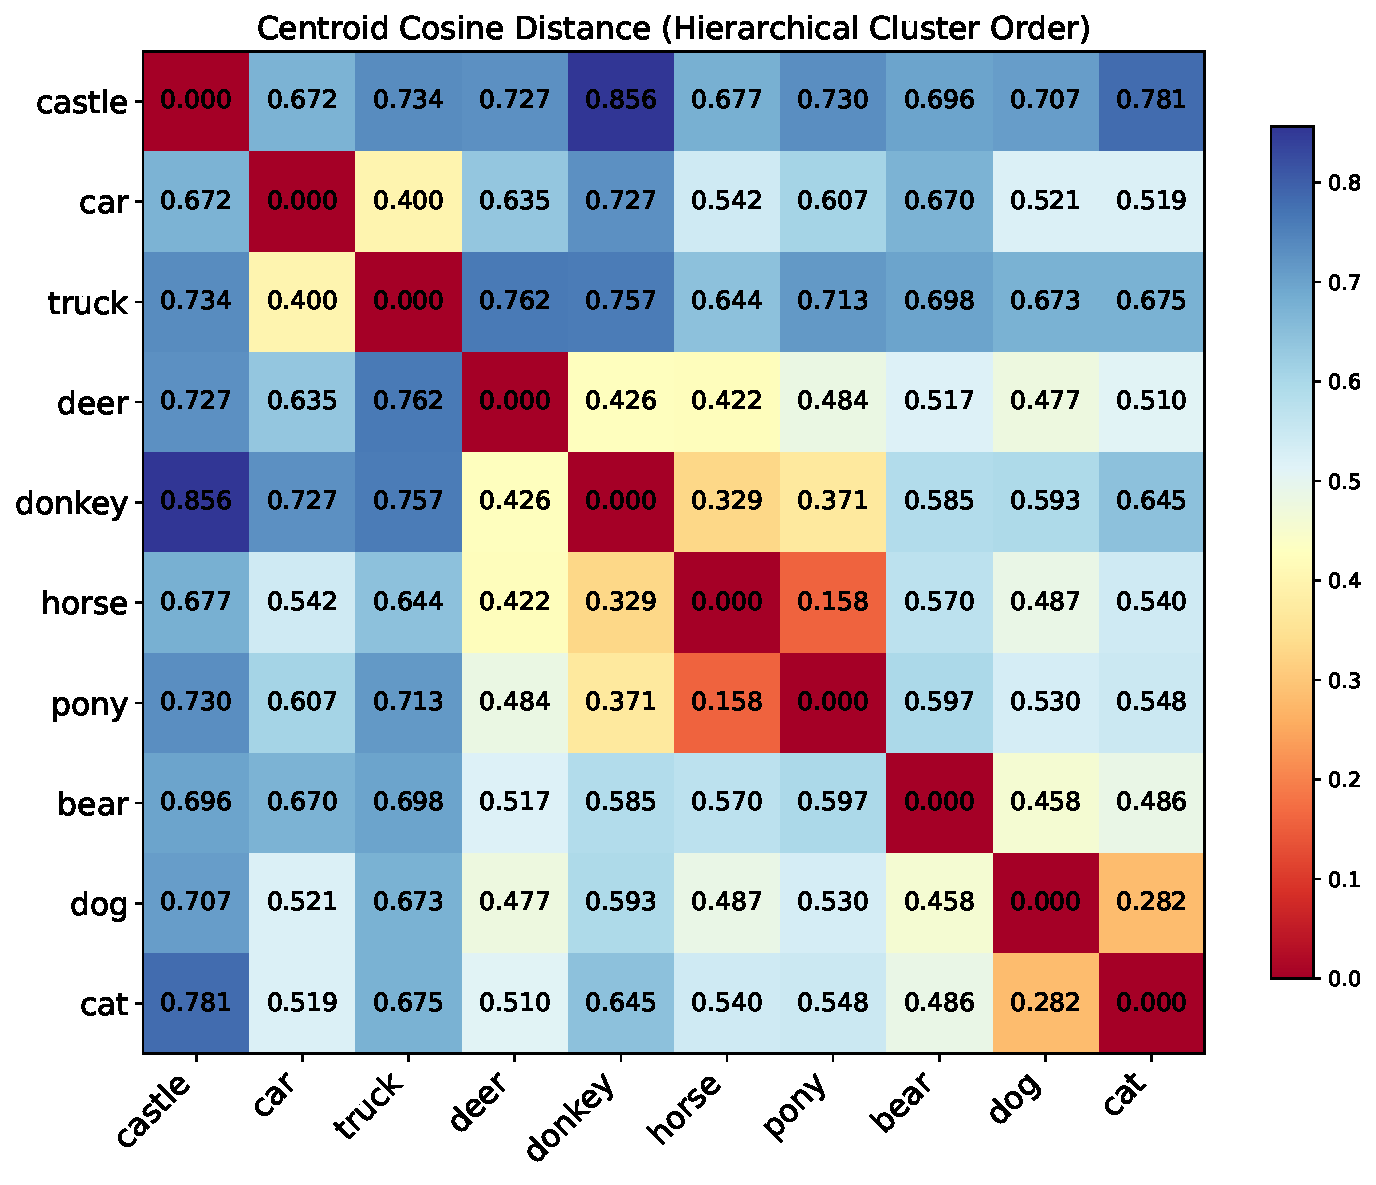
\includegraphics[width=0.75\linewidth]{img/centroid_distance_clustered_mid.pdf}
\caption{
Pairwise centroid cosine distance between concept activation regions at \texttt{mid\_block.attentions.0}, ordered by hierarchical clustering. Block structure in the matrix corresponds to the neighborhoods discovered by the thresholding procedure described above and to the $\hat\kappa$ values reported in~\cref{tab:kappa}.
}
\label{fig:distance_matrix}
\end{figure}

\paragraph{On the use of centroid distance as a proxy.}
The centroid cosine distance plays a different role from $\hat\kappa$ itself, and the two should not be conflated. 
\Cref{def:overlap} is stated in terms of the volume of fattened activation regions, whose membership is determined by an \emph{infimum} over per-sample distances (the closed $\rho$-neighborhood $\mathcal{R}_c^{(\rho)}$). The centroid, by contrast, is a single \emph{average} summary of each region.

Centroid distance is used only for \emph{neighborhood discovery} (\cref{def:semantic_neighborhood}), an upstream step of deciding which pairs of concepts are close enough to warrant an overlap measurement. We use it here for two reasons. First, it is a stable summary statistic that degrades gracefully under the finite-sample, high-dimensional regime in which we estimate activation regions.
Second, an outlier-robust statistic at this stage is conservative: a concept that is filtered {out} of $\mathcal{N}(c_u)$ contributes zero to the resulting estimator, so under-inclusion only weakens the bound. The estimator $\hat\kappa$ is therefore a lower bound on $\kappa(c_u, \rho)$ both because $\mathcal{N}(c_u) \subseteq \mathcal{C} \setminus \{c_u\}$ and because the discovery step itself is conservative. Empirical comparisons against the bound of~\cref{thm:tradeoff} therefore remain valid.

The $\hat\kappa$ statistic itself does not use centroid distance. As specified in the overlap estimation step above, $\hat\kappa$ is computed via a nearest-neighbor estimator: for each activation sample $\mathbf{a} \in \mathcal{S}_{c_u}$, we check whether there exists \emph{any} sample $\mathbf{b}$ from \emph{any} concept in $\mathcal{N}(c_u)$ with $d_{\cos}(\mathbf{a}, \mathbf{b}) \le \rho$.
This is the natural finite-sample analogue of the fattened-region membership condition $\mathbf{a} \in \mathcal{R}_{c'}^{(\rho)}$ (with the radius $\rho$ converted to cosine units, see ``On the relationship between cosine and $\ell_2$ metrics'' above), and the fraction of target samples satisfying this condition is a Monte Carlo estimate of the volume ratio in~\cref{def:overlap} restricted to $\mathcal{N}(c_u)$. The centroid-distance visualization in~\cref{fig:distance_matrix} therefore serves only as an auxiliary consistency check: blocks of small centroid distance should coincide with the discovered $\mathcal{N}(c_u)$, and the high-$\hat\kappa$ targets should sit inside such blocks.

\paragraph{Interpretation.}
Under this estimator, $\hat\kappa(c_u) \in [0, 1]$ captures the sample-level  coverage of the target region by its neighbors. The results in~\cref{tab:kappa} exhibit a bimodal structure. The four animal-subtype concepts embedded in dense semantic neighborhoods, \texttt{dog} ($\hat\kappa = 0.89$), \texttt{bear} ($\hat\kappa = 0.82$), \texttt{horse} ($\hat\kappa = 0.81$), and \texttt{cat} ($\hat\kappa = 0.77$), exhibit the  highest overlap, consistent with their small inter-centroid distances to fine-grained subtypes (\cref{fig:distance_matrix}). 
Under our procedure, these concepts each have multiple discovered neighbors, and individual samples from these neighbors fall within the fattening radius $\rho$ of a substantial fraction of target samples. The high overlap is also \emph{robust} to which neighbors are included: in the \texttt{horse} pool, several individual neighbors (\texttt{mare}, \texttt{pony}, \texttt{stallion}) each cover 60--80\% of target samples on their own, and the union across all seven discovered neighbors saturates at $\hat\kappa = 0.81$, indicating that overlap is supported by a representational manifold shared across the equine subtype family rather than driven by a single sensitive neighbor choice.

The architectural concept \texttt{castle}, by contrast, exhibits substantially lower overlap ($\hat\kappa = 0.27$) despite having six discovered neighbors within $\delta$. The distinction is qualitative: castle's neighbors are semantically related but represent \emph{distinct} architectural types rather than fine-grained subtypes of a shared category. They occupy nearby but non-overlapping regions of activation space, so the centroid distances cross the $\delta$ threshold while individual sample-level overlap remains limited. Controls like \texttt{jellyfish}, \texttt{melon}, \texttt{police car} are correctly filtered out by the $\delta$ step across all five targets and contribute zero to $\hat\kappa$, confirming that the estimator is not driven by pool-wide sample density.

This bimodal structure, high-$\hat\kappa$ animal subtypes clustered in $[0.77, 0.89]$ and moderate-$\hat\kappa$ architecture at $0.27$ reflects a property of the model's internal representations at the probed layer: text-to-image diffusion models represent fine-grained subtypes of a common taxonomic category (breeds of dog, equine subtypes) as overlapping regions of a shared activation manifold, while distinct-but-related concepts in other domains maintain more separable representations. \Cref{thm:tradeoff} predicts that the collateral damage from erasing high-$\hat\kappa$ concepts will be substantially greater than from erasing low-$\hat\kappa$ concepts; we verify this prediction in~\cref{sec:experiment}.

% \paragraph{Robustness to metric and estimator choice.}
% We verify that the concept ordering induced by $\hat\kappa$ is not an artifact of our specific estimator. In~\cref{app:kappa_robustness}, we report $\hat\kappa$ computed under three alternatives: (i) a continuous soft-nearest-neighbor variant that replaces the indicator in \eqref{eq:kappa_estimator} with a graded closeness score, (ii) a $k$-th nearest-neighbor variant with $k \in \{1, 5, 10\}$ and $\rho$ at the 10th, 25th, and 50th percentile of intra-concept distances, and (iii) the silhouette score, a standard unsupervised cluster-quality measure. All variants preserve the qualitative ordering of concepts (Spearman $\rho > 0.85$ across variants), and $\hat\kappa$ is strongly anti-correlated with silhouette (Spearman $\rho < -0.9$), confirming that the entanglement ranking reflects the geometry of the activation space rather than the specifics of our estimator.

\subsection{Per-Target Results}
\label{app:kappa_per_target}
We apply the procedure of~\cref{app:kappa_estimation} to the five target concepts used throughout~\cref{sec:experiment}. The shared candidate pool $\mathcal{C}_{\mathrm{pool}}$ consists of concepts spanning all five target domains and an out-of-domain control set: the five targets themselves; their respective fine-grained subtype candidates (equine, feline, canid, ursine, architectural); and ten generic out-of-domain controls (\texttt{airplane}, \texttt{bicycle}, \texttt{cactus}, \texttt{jellyfish}, \texttt{lighthouse}, \texttt{melon}, \texttt{police car}, \texttt{teapot}, \texttt{violin}, \texttt{volcano}). 
\Cref{tab:kappa_per_target} reports the resulting $\hat\kappa$ values together with the size of each discovered neighborhood $|\mathcal{N}(c_u)|$ (\cref{def:semantic_neighborhood}), the per-target fattening radius $\rho_{c_u}$, and the discovered neighbors.

\begin{table}[ht]
\centering
\small
\setlength{\tabcolsep}{6pt}
\begin{tabular}{lcccl}
\toprule
\textbf{Target} & $\hat\kappa$ & $|\mathcal{N}(c_u)|$ & $\rho_{c_u}$ & \textbf{Discovered neighbors} \\
\midrule
\texttt{dog}    & 0.89 & 5 & 0.13 & puppy, labrador, husky, beagle, retriever \\
\texttt{bear}   & 0.82 & 5 & 0.14 & grizzly, panda, polar bear, koala, cub \\
\texttt{horse}  & 0.81 & 7 & 0.15 & pony, mare, donkey, stallion, foal, zebra, mule \\
\texttt{cat}    & 0.77 & 5 & 0.15 & kitten, lynx, leopard, tiger, cheetah \\
\texttt{castle} & 0.27 & 6 & 0.18 & fortress, palace, citadel, keep, manor, cathedral \\
\bottomrule
\end{tabular}
\caption{
\textbf{Per-target $\hat\kappa$ estimation results.} For each target $c_u$, we report the estimated entanglement coefficient $\hat\kappa$, the number of discovered neighbors within the centroid-distance threshold $\delta$, the fattening radius $\rho_{c_u}$ (median intra-concept cosine distance), and the discovered neighbor set. \texttt{castle} has a discovered neighborhood of comparable size to the animal targets but $\hat\kappa$ roughly $3\times$ lower, isolating semantic density rather than neighborhood cardinality as the driver of $\hat\kappa$. }
\label{tab:kappa_per_target}
\end{table}

\paragraph{Per-neighbor coverage decomposition.}
For \texttt{horse}, the per-neighbor coverage of target samples (fraction of $\mathcal{S}_{\texttt{horse}}$ with a within-$\rho$ activation in the neighbor's sample set) decomposes as: \texttt{mare} ($0.78$), \texttt{pony} ($0.72$), \texttt{stallion} ($0.66$), \texttt{donkey} ($0.41$), \texttt{foal} ($0.38$), \texttt{zebra} ($0.30$), \texttt{mule} ($0.22$), with the union saturating at $\hat\kappa = 0.81$. 
The strongest individual neighbors (\texttt{mare}, \texttt{pony}) already cover most of the target region on their own, and several others contribute substantially, indicating that overlap is supported by a representational manifold shared across the equine subtype family rather than being sensitive to which specific neighbor is picked. By contrast, \texttt{castle}'s six discovered neighbors each cover only $0.05$--$0.12$ of the target region, and their union saturates at $\hat\kappa = 0.27$, consistent with castle's neighbors representing distinct architectural types rather than fine-grained subtypes of a shared category.

 

\subsection{Sensitivity of $\hat\kappa$ to the choice of probe layer}
\label{app:layer_sensitivity}

The $\hat\kappa$ estimator fixes the probe layer at $\ell^* = \texttt{mid\_block.attentions.0}$. To assess whether the bimodal $\hat\kappa$ structure reported in~\cref{tab:kappa} is an artifact of this choice, we re-ran the estimator at four additional cross-attention layers spanning the U-Net depth, holding all other estimator hyperparameters (candidate pool $\mathcal{C}_{\text{pool}}$, $\delta$-threshold percentile, fattening radius rule, prompt templates, timestep $t^*=25$) fixed.

\begin{table}[ht]
\centering
\small
\setlength{\tabcolsep}{2pt}
\begin{tabular}{lccccc|cc}
\toprule
\textbf{Layer} & \texttt{castle} & \texttt{cat} & \texttt{horse} & \texttt{bear} & \texttt{dog} & Spearman $\rho$ vs.\ mid & Animal std \\
\midrule
\texttt{down\_blocks.2.attentions.1} & 0.26 & 0.71 & 0.74 & 0.87 & 0.85 & $+0.90$ & 0.069 \\
\textbf{\texttt{mid\_block.attentions.0}} & \textbf{0.27} & \textbf{0.77} & \textbf{0.81} & \textbf{0.82} & \textbf{0.89} & --- & \textbf{0.043} \\
\texttt{up\_blocks.1.attentions.0} & 0.09 & 0.59 & 0.48 & 0.88 & 0.79 & $+0.80$ & 0.158 \\
\texttt{up\_blocks.1.attentions.1} & 0.39 & 0.36 & 0.61 & 0.91 & 0.76 & $+0.80$ & 0.203 \\
\texttt{up\_blocks.2.attentions.0} & 0.00 & 0.78 & 0.63 & 0.89 & 0.88 & $+0.80$ & 0.105 \\
\bottomrule
\end{tabular}
\caption{\textbf{$\hat\kappa$ across five candidate probe layers.} All four alternative layers produce a $\hat\kappa$ ranking strongly consistent with mid-block (Spearman $\rho \geq 0.80$). Mid-block additionally yields the tightest cluster of animal-subtype $\hat\kappa$ values (std $=0.043$, vs.\ $0.069$--$0.203$ elsewhere), making it the layer at which the ``animal-subtype shared-manifold'' structure is most coherently expressed.}
\label{tab:layer_sensitivity}
\end{table}

\paragraph{Conclusion.} Three observations support our default choice. First, the $\hat\kappa$ \emph{ranking} of the five target concepts is stable across all probed layers (Spearman $\rho \geq 0.80$ vs.\ mid-block in every case): the ordering $\hat\kappa(\texttt{castle}) \ll \hat\kappa(\{\texttt{cat}, \texttt{horse}, \texttt{bear}, \texttt{dog}\})$ is a property of the underlying concept geometry, not of mid-block specifically. Second, mid-block produces the cleanest bimodal separation between high-entanglement animal subtypes and the low-entanglement architectural concept: the smallest animal $\hat\kappa$ exceeds $\hat\kappa(\texttt{castle})$ by $0.50$ at mid-block, vs.\ $0.39$--$0.45$ at down-block / up-block-1.0 and an inverted ordering at up-block-1.1 where $\hat\kappa(\texttt{castle}) = 0.39 > \hat\kappa(\texttt{cat}) = 0.36$. Third, mid-block has the lowest within-cluster spread among the four animal concepts (std $0.043$, less than half that of every up-block layer), consistent with mid-block being the layer at which fine-grained subtypes are most coherently represented as overlapping regions of a shared manifold. We therefore use mid-block as the default probe for $\hat\kappa$ estimation, the visualization in~\cref{fig:umap}, the Lipschitz checks in~\cref{app:lipschitz}, and the within-target displacement validation in~\cref{app:displacement}.

\paragraph{A note on \texttt{up\_blocks.1.attentions.1}.} The direct displacement measurements in~\cref{app:displacement_kappa} are reported at \texttt{up\_blocks.1.attentions.1} rather than mid-block. The $\hat\kappa$ ranking at this layer agrees with mid-block (Spearman $\rho = 0.80$, supporting the cross-target $\hat\kappa$-scaling reported there), but its bimodal separation is the weakest of the five layers. We use this up-block layer for direct displacement specifically because it lies downstream of the cross-attention edits applied by fine-tuning methods and therefore exhibits the largest absolute displacement signal under STEREO and AdvUnlearn; the $\kappa$-scaling claim in~\cref{app:displacement_kappa} relies on the Spearman ranking, which is preserved, not on the absolute $\hat\kappa$ values at that layer.